\documentclass[12pt,a4paper]{article}
\usepackage[left=2.5cm,right=2.5cm,top=2.5cm,bottom=2.5cm,footskip=2cm,headheight=1.5cm]{geometry}
\usepackage[utf8]{inputenc}
\usepackage{amssymb,booktabs,mathtools}
\usepackage{ dsfont }
\newcommand{\tallstrut}{\vphantom{\frac{5_A}{4,10^3}}}
\usepackage{wrapfig}
\setlength{\parskip}{0.4em}

\title{Planetary Astrophysics}
\author{Athos Silva}
\date{2020}

\usepackage{natbib}
\usepackage{graphicx}

\begin{document}

\maketitle
\tableofcontents
\pagebreak
\section{Exoplanet detection (March 13th)}

The first exoplanetary detection method was the radial velocity. It is done by obtaining the redshift of the star caused by the solar system's gravitation dynamics around its baricenter. It provides information about the planet's semi-major axis (from the orbital period), mass (from the amplitude of the velocity curve) and eccentricity (from the light curve). Solar spots can result in a false positive because they can simulate a redshift which is not caused by the orbit but by obscuring the incoming or outgoing rays due to the rotation of the star.

Transit method is done by observing the amount of blocked radiation due to the passage of a planet in front of a star's line of sight. It allows us to measure the radius of the planet from the amount of blocked radiation and the the semi-major axis from the time of transit.

In the Microlensing method we observe the magnification due to the relativistic curvature of light from a radiation source by the transit of a star and its orbiting planet. It's not a practical method as it is only possible to observe once and it does not happen often.

Astrometry method is similar to the radial velocity, but instead of redshift we measure the displacement of the star due to its solar system's gravitational dynamics. It is a harder method because it's not possible to do it in terrestrial observations.

Direct imaging method resorts to masking the starlight and observing the radiation from young hot planets orbiting around.

Thanks to technical limitations, massive planets are easier to be detected, which rises a bias towards a bigger number of discoveries of this kind of planets in comparison to others. The radial velocity method is better observed on planets in distant orbits since they cause a bigger wobble on the star, and transit method is better observed on planets with smaller orbits since they often have lower eccentricity which reflects in higher chances to transit in front of the star's line of sight.

We can use radial velocity and transit simultaneously to obtain the planet's mass and radius, with such we can derive the density and then assume its composition. When doing RV method, detecting a peak in the RV indicates the presence of an obscuring, transiting planet thanks to a similar effect caused by black spots. From the shape of the peak we can also obtain the planet's inclination of the orbital plane in relation to the star's rotation axis.

Terrestrial, Earth and Super-Earths: 
\begin{itemize}
    \item Mass range: 1-15 Earth masses;
    \item Composition: high density materials (rocky with water, ice or atmosphere);
    \item Frequency of appearance: 30-50\%;
    \item No correlation with star's metallicity;
    \item Many hot planets and all ranges of eccentricity.
\end{itemize}

Debris disks have more luminousity than planets because of its larger area. Their presence can indicate the presence of planetesimals and planets, since they depend of recent collisions otherwise they are swallowed by the star and disappear. The shape and presence of structures in these disks can also indicate presence of planets.

The classic planetary system formation model could not explain the existence of hot Jupiters, which demanded some new explanations for the gaps in the model. 

Planet migration is divided in types I, II and III. 

Type I happens to planets with smaller masses, and it is caused either by wakes, which resulting forces carry the planet inwards, or the horseshoe torque, which pushes it outwards. Wakes are produced by resonance of the planetesimal orbit with disk rings which share an orbit ratio described by integers (1:2, 1:4, etc). Horseshoe is caused by an U-turn motion pattern whenever particles in orbit come close to the planetesimal.

Type II affect giant planets. They create a ring of gap in the disk around its orbit, which provokes an inwards migration whose speed depends on the dust viscosity.

The presence of pebbles can explain how planets can be formed so fast before the extinction of the disk.

The fact that Jupiter and Saturn did not migrate can be explained by Saturn migrating inwards faster than Jupiter and locking both in a resonating motion.

Planet-planet scattering is caused by mutual perturbations among the orbit of planets, resulting in the ejection of a planet out of the system and planets with small orbits with high eccentric orbits and tidal effects.
\vspace{5mm}

\section{Earth's Magnetic Field (March 17th)}

The composition of the mantle and nucleus of Earth is done by seismography. When shock waves travel through the layers from above and hit another part of the crust, the delay between waves due to the different composition is calculated and from that the components are inferred.

The bigger radial increase of pressure towards the center compared to the increase of temperature is the reason why the nucleus is solid.

The flip in the magnetic poles of Earth was discovered by analysing the layers of volcanic rocks, which registered the direction of Earth's field at the time it was erupted.
The source of Jupiter and Saturn's magnetic field is attributed to the high pressure in the gas cloud, which causes the metallic hydrogen to leave its electrons run free. Uranus and Neptune's source of magnetic field is still unknown.

The magnetic field along the radial components is given by:
\begin{equation}
\begin{split}
&B_r=\frac{2\mu_0m}{4\pi^3}cos\alpha \\
&B_\alpha=\frac{\mu_0m}{4\pi^3}sin\alpha \\
&B_\phi=0
\end{split}
\end{equation}
\[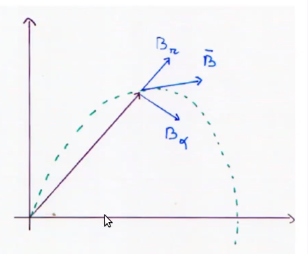
\includegraphics[scale=0.85]{1}\]
where $\alpha$ is 0 at the north pole and $\phi$ is the angle which plane is perpendicular to $\alpha$'s plane. But using the geology's system of latitude, with $\theta$ as 0 at the equator, and considering the field to be negative because it is inverted to the geographic poles:
\begin{equation}
\label{2}
\begin{split}
&B_r=-\frac{2M_B}{r^3}sin\theta \\
&B_\theta=\frac{M_B}{r^3}cos\theta \\
&B_\phi=0 \\
&M_B=7,906\cdot10^{15}\ T\;m^3=\frac{\mu_0m}{4\pi}
\end{split}
\end{equation}
\[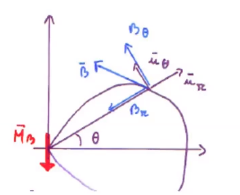
\includegraphics[scale=1.25]{2}\]
the magnetic field line is: \\
\begin{equation}
    r(\theta)=r_ecos^2(\theta)
\end{equation} \\
where $r_e$ is the radius at the equator ($\theta=0$). To prove that this is indeed the line function, we can applying it to the velocity vector and show that it is tangent to B: 
\begin{equation}
\label{4}
\begin{split}
    &\textbf{v}=\dot{r}û_r+r\frac{d\theta}{dt}û_\theta \\
    &\textbf{v}=-2r_ecos(\theta)sin(\theta)\frac{d\theta}{dt}û_r+r_ecos^2(\theta)\frac{d\theta}{dt}û_\theta \\
    &\textbf{v}=r_ecos(\theta)\frac{d\theta}{dt}(-2sin\thetaû_r+cos\thetaû_\theta)
\end{split}
\end{equation} 
the last term in the last line of \eqref{4} is responsible for the directions thanks to the unit vectors. This term is similar to the one in the vector B in eq.\eqref{2}, so we can assume B and \textbf{v} to be parallel to each other and \textbf{v} is tangent at any point of $r(\theta)$. The magnitude of B is: \\
\begin{equation}
    |B|=\sqrt{(-\frac{2M_B}{r^3}sin\theta)^2+(\frac{M_B}{r^3}cos\theta)^2}=\frac{M_B}{r^3cos^6\theta}\sqrt{-4sin^2\theta+cos^2\theta}
\end{equation} \\
in the equator ($\theta=0$) we have: \\
\begin{equation}
\label{6}
    |B|=\frac{M_B}{r^3}
\end{equation} \\
which indicates that B drops down very fast with the cube of radius.

Unperturbed motion: characterized by the cyclotron motion of charged particles along the magnetic field of Earth. Considering vector B to be present only on the z-axis ($\textbf{B}=(0,0,\textit{B})$) and vector v to be dimensional on the xy plane ($\textbf{v}=(\textit{$v_x$},\textit{$v_y$},0)$):
\begin{equation}
\begin{split}
m\Ddot{x}&=qB\dot{y} \\ m\Ddot{y}&=qB\dot{x} 
\end{split}
\end{equation}
deriving equations and substituting $\Ddot{x}$ and $\Ddot{y}$:
\begin{equation}
    \begin{split}
        \dddot{x}&=\frac{qB}{m}\Ddot{y}=-(\frac{qB}{m})^2\dot{x} & \dddot{y}&=\frac{qB}{m}\Ddot{x}=-(\frac{qB}{m})^2\dot{y}
    \end{split}
\end{equation}
integrating the x and y equations we get:
\begin{equation}
\begin{split}
\Ddot{x}=-\Omega_c^2x \\
\Ddot{y}=-\Omega_c^2y \\
\end{split}
\end{equation}
\begin{equation}
    \Omega_c=\frac{qB}{m}
\end{equation}
where $\Omega_c$ is the called \textit{cyclotron frequency}. Cyclotron (or Larmor) radius is obtained from it:
\begin{equation}
\begin{split}
\label{11}
    |a|=\Omega_c^2|r|=\frac{v^2}{r} \\
    \Omega_c^2=\frac{v^2}{r^2}{\implies}r=\frac{v_{\bot}m}{qB}
\end{split}    
\end{equation}
The drift motion, which causes the particles to move sideways, is due to a) inconstancy of the field along the coil-shaped lines; b) inconstancy of the field along Earth's radius; c) presence of electric and gravitational fields. The drift velocities are:
\begin{align}
    \label{12}
    a){\quad}v_D^\|&=mv_\|^2\frac{B{\times}n}{R_cqB^2} & \textrm{where }R_c=\frac{B}{\nabla_\|B} \\
    b){\quad}v_D^\bot&=\frac{1}{2}mv^2_\bot\frac{B\times{\nabla}{\cdot}B}{qB^2} \\
    \label{14}
    c){\quad}v^E_D&=\frac{E\times B}{B^2} & v^G_D=\frac{G\times B}{qB^2}
\end{align}
where $v_\|$ and $v_\bot$ are respectively the parallel and perpendicular components of the particle's velocity. The mean motion vector \textbf{n} and the gradient of the field $\nabla\cdot\textbf{B}$ are both pointing approximately towards the center of Earth, therefore we infer the same for $v_D^\|$ and $v_D^\bot$'s directions, consequently allowing us to sum up both of them together. $R_c$ is the \textit{curvature radius}. Considering that the magnetic field is much more dominant than the electric and gravitational ones, the drift from c) has much lower in magnitude. Also, the drift from b) is more intense than a)'s because $v_\bot$ is higher than $v_\|$. 

To prove the drift velocity equations we start from the electric field drift \eqref{14}. Assuming that we consider the axis, around which the cyclotron motion happens, is moving sideways instead of the particle, we consider particle's velocity as:
\begin{equation}
\label{15}
    \textbf{u}=\textbf{v}-\frac{\textbf{E}\times\textbf{B}}{B^2}
\end{equation}
since B and E are constants, deriving the equation provides:
\begin{equation}
    \frac{d\textbf{u}}{dt}=\frac{d\textbf{v}}{dt}
\end{equation}
multiplying by mass we obtain the Lorentz force:
\begin{equation}
    m\frac{d\textbf{u}}{dt}=m\frac{d\textbf{v}}{dt}=q(\textbf{E}+\textbf{v}\times\textbf{B})
\end{equation}
substituting v from eq. \eqref{15}:
\begin{equation}
\begin{split}
    m\frac{d\textbf{v}}{dt}&=q(\textbf{E}+\textbf{u}\times\textbf{B}+\frac{(\textbf{E}\times\textbf{B})\times\textbf{B}}{B^2}) \\
    &=q(\textbf{E}+\textbf{u}\times\textbf{B}-\frac{\textbf{E}(\textbf{B}\cdot\textbf{B})}{B^2}+(\textbf{E}\cdot\textbf{B})\frac{\textbf{B}}{B^2}) \\
    &=q(\textbf{u}\times\textbf{B}+\textbf{E})
\end{split}   
\end{equation}
the electric field term in the end is on the parallel direction to B (due to the scalar product with B) which is irrelevant to the drift, so we ignore it. The result is equal to the gyro motion of the particle with no drift, acting in the perpendicular plane, which indirectly proves our formula for $v^E_D$:

\begin{equation}
    m\frac{d\textbf{u}_\bot}{dt}=q(\textbf{u}\times\textbf{B})
\end{equation}
having proved $v^E_D$, we take multiply it by q/q to obtain a general formula for the drift:
\begin{equation}
\label{20}
    v_D=\frac{\textbf{E}\times \textbf{B}}{B^2}=\frac{q\textbf{E}\times\textbf{B}}{qB^2}=\frac{\textbf{F}\times \textbf{B}}{qB^2}
\end{equation}
which is similar to the gravitational drift if we consider the force to be from gravity. Now from \eqref{20} we get to \eqref{12} by the centrifugal force in the mean motion direction, which is given as:
\begin{align}
\begin{split}
    \textbf{F}=-\frac{mv^2_\|}{R_c}\hat{n} \\
    v_D=-mv^2_\|\frac{\textbf{n}\times\textbf{B}}{R_cqB^2}
\end{split}
\end{align}

The mirror motion is responsible for making the charged particles turn around when they reach the magnetic poles. It happens because of the concentration of field lines in both areas. We use the adiabatic invariant to approach this question, which assumes that said invariant (magnetic moment $\mu$) is constant considering that the parameters in the system change very slowly (field lines). 
\vspace{10mm}

\section{Earth's Magnetic Field (March 20th)}

Starting from the assumption that the rotating ion is a current I around an area A, this is the result of the adiabatic invariant magnetic moment in relation to the mass, field and parallel velocity:
\begin{align}
\begin{split}
\label{22}
    &\mu=IA_s=\frac{dq}{dt}\pi R_c^2=\frac{Q}{T}\pi R_c^2 \\
    &\Omega_c T=2\pi \implies \frac{Q}{2\pi}\Omega_c\pi R_c^2=\frac{Q}{2}\Omega_c R_c^2 \\
    &\Omega_c=\frac{qB}{m}\implies\frac{Q}{2}\frac{QB}{m}R_c^2 \\
    &\Omega^2r^2=v^2\implies\frac{Q}{2}\frac{QB}{m}\frac{v^2m^2}{Q^2B^2}= \frac{1}{2}m\frac{v_\bot^2}{B}
\end{split}
\end{align}
from the Lorentz force, multiplying both hands by \textbf{v}:
\begin{align}
\begin{split}
    &\textbf{v}\frac{d}{dt}(m\textbf{v})=\textbf{v}Q\,(\textbf{E}+\textbf{v}\times\textbf{B}) \\
    &\frac{d}{dt}(\frac{1}{2}m\textbf{v}^2)=Q\textbf{v}\cdot\textbf{E}
\end{split}
\end{align}
which express the kinetic energy variation $\Delta E_K$. If we consider the field line flux to be increasing, we could say we have the direction of \textbf{E} as negative to \textbf{v}, but considering a negative charge Q, the total variation of kinetic energy would amount as positive, i.e. increasing. Integrating and then using Faraday's law, we obtain:
\begin{align}
    \begin{split}
        &\int_T d(E_K)=Q\int_T \textbf{E}\cdot\textbf{v}dt \\
        &v=\frac{dl}{dt}\implies Q\oint_T \textbf{E}\cdot\textbf{dl}=-Q\int\frac{dB}{dt}dS
    \end{split}
\end{align}
which represents the change in magnetic field. Since the field varies slowly, we can write:
\begin{align}
    &-Q\int\frac{dB}{dt}dS=\frac{dB}{dt}\pi R^2_c
\end{align}
taking $\Delta E$ as an expression of B:
\begin{align}
    \begin{split}
        &\Delta E_K=Q\frac{dB}{dt}\pi R^2_c \\
        &\Omega^2r^2=v^2\implies Q\frac{\Delta B}{T}\pi\frac{v^2}{\Omega^2} \\
        &\Omega_c T=2\pi\quad\textrm{and}\quad\Omega_c=\frac{qB}{m}\implies Q\frac{\Delta B}{2\pi}\frac{QB}{m}\pi\frac{v^2}{Q^2B^2}m^2=\frac{1}{2}mv^2\frac{\Delta B}{B}=E_K\frac{\Delta B}{B}
    \end{split}
\end{align}
we then conclude that $\Delta E_K$ is equal to itself times the increasing percentage of \textbf{B}. Now, we calculate the variation in the ratio between kinetic energy and magnetic field $E_K/B$:
\begin{align}
    \begin{split}
        \Delta(\frac{E_K}{B})&=\frac{\partial(\frac{E_K}{B})}{\partial E_K}\cdot\Delta E_K+\frac{\partial(\frac{E_K}{B})}{\partial B}\cdot\Delta B \\
        &=\frac{1}{B}\Delta E_K-\frac{E_K}{B^2}\Delta B \\
        &=\frac{1}{B}\frac{E_K\Delta B}{B}-\frac{E_K}{B^2}\Delta B \\
        &=0
    \end{split}
\end{align}
which allows us to conclude that $\mu$ is an adiabatic invariant. 

Looking back at $\mu$ in eq.\eqref{22}, and remembering the relation of $\Omega_c$ with the radius \eqref{11}, we conclude that the last one is inversely proportional to \textbf{B} ($r\:\alpha\:1/\sqrt{B}$), and so the closer to the poles, where the field is more intense, the smaller the particle's radius of rotation.

Lastly, if we take in mind that the total kinetic energy of the particle is given by both parallel and perpendicular velocities:
\begin{align}
    E=\frac{1}{2}m(v^2_\|+v^2_\bot)
\end{align}
and that $\mu$ is always constant, therefore the variables $v_\bot$ and \textbf{B} must increase proportionally, and finally, according to \eqref{22}, the velocity must increase by the square while \textbf{B} increases linearly, we find that, considering that we do not have production of work in the magnetic field and we also maintain the total kinetic energy as constant, while $v_\bot$ increases exponentially towards the pole, $v_\|$ must decrease in the same rate, causing the particle to halt and turn back.

We can also see the mirror motion being caused by the inclination of field lines towards the poles, which produces a component of the force in the opposite direction of the parallel speed.

Van Allen belts are composed by the currently studied charged particles, which make a coil-shaped cloud around the Earth. The inner belt is 1-3 Earth radius large and is composed by positively charged ions, while the outer one is 3-9 $R_E$ large and dominated by electrons. Satellites are usually concentrated in an orbit between both belts where the density of particles is the lowest, while space telescopes are sent to orbits outside the outer belt so that the electrons do not interfere with observations. In order to change orbits of different radius, the spacecrafts can turn on the engines to move radially out or inwards.

The South Atlantic anomaly is caused by the inclination difference between Earth's rotation axis and the magnetic poles, which cause the particle belts to get closer to the surface.

Jupiter has an anomalous north pole, which is speculated to be caused by metallic hydrogen. Plus, the volcanic activity of its satellite, Io, ejects clouds in its own orbit, which creates a torus that is ionized and spread by the sunlight.

The magnetosphere of Earth can be seen as a shield that ejects solar winds out of the planet's direction. To calculate the pressure exerted by the winds we start from the kinetic theory of the gases, where we consider the change of momentum of a gas particle due to collision. Imagining that the particle is perfectly deflected, momentum change is:
\begin{align}
    \Delta p=-2mv_x
\end{align}
if we consider that the particle travels all the length \textit{l} inside a box, is reflected and reaches its initial point then the travel time \textit{t} is:
\begin{align}
    t=\frac{2l}{v_x}
\end{align}
relating the force of all particles (total of N) with the time, and then the pressure with the force:
\begin{align}
    &F=\frac{N\Delta p}{t}=\frac{2Nmv_x^2}{2l}=\frac{Nmv^2_x}{l} \\
    &P=\frac{F}{l^2}=\frac{Nmv^2_x}{l^3}
\end{align}
now relating density $\rho$ with pressure, and assuming that the particle's motion is random:
\begin{align}
    \rho=\frac{Nm}{V}\implies P=\rho v_x^2=\frac{1}{3}\rho v^2
\end{align}
where v is the average quadratic velocity. Since the solar wind is only moving in one direction, which is the one towards Earth, we don't need to account for contributions from other dimensions, so multiply the formula by 3 and obtain $P=\rho v^2$. Opposed to the wind pressure, there is the magnetic pressure:
\begin{align}
    P=\frac{1}{2}\frac{B^2}{\mu_0}
\end{align}
which has indeed the same dimension as pressure ($\rho_E\Leftrightarrow\frac{Newton\cdot meter}{meter^3}=\frac{Newton}{meter^2}\Leftrightarrow P$), and is the same as the disruptive force of a magnetic field in a solenoid. Equalizing both pressures, substituting \eqref{6} and then deriving the magnetosphere's mean radius $R_M$ from it: 
\begin{align}
\begin{split}
    &\rho v^2=\frac{1}{2}\frac{M_B^2}{r^6}\frac{1}{\mu_0} \\
    &R_M=(\frac{1}{2\mu_0}\frac{M_B^2}{\rho v^2})^{1/6}
\end{split}
\end{align}
from which, using reasonable data, it is assumed to be roughly 10 $R_E$ and covers the whole outer belt.

The quantity of neutrinos measured from the Sun through chemical reaction were at first only about 40\% from the expected, but only electron neutrinos were detected, while there are still the muon and tau neutrino and all three are interchangeable.

The solar winds are known for having many bursts in a very short time spam. Their speeds are higher at the poles and lower at the equator, but density works in the opposite way. The magnetic pole inversion cycle of the Sun (Maunder cycle) is much faster than Earth's and takes only about 11 years. During this period, there is an increasing magnetic activity and appearances of black spots, flares and coronal mass ejections, which quickly drop down to minimum after the end of the cycle.
\vspace{10mm}

\section{Sun's Magnetic Field/Non-gravitational Forces (March 24th)}

We start assuming that the plasma is emitted with velocity \textbf{u} from the surface of the Sun (which spins with angular velocity $\Omega$). The components in r, $\theta$ and $\phi$ are:
\begin{align}
    \begin{split}
    \textbf{u}\;
    \begin{cases}
        u_r=u \\
        u_\theta=0 \\
        u_\phi=-\Omega_rsin\theta
        \end{cases}
    \end{split}
\end{align}
The general velocity vector in polar coordinates is given as:
\begin{align}
\label{37}
    \textbf{v}=\dot{r}ê_r+r\dot{\theta}ê_\theta+rsin\theta\dot{\phi}ê_\phi
\end{align}
if we equalize the rate between the radial and azimuthal terms of \textbf{v} with the same rate from \textbf{u}:
\begin{align}
\begin{split}
\label{38}
    \frac{\dot{r}}{rsin\theta\dot{\phi}}&=\frac{u}{-\Omega rsin\theta} \\
    \frac{\dot{r}}{\dot{\phi}}&=\frac{dr}{dt}\frac{dt}{d\phi}=\frac{u}{-\Omega} \\
    r(\phi)&=-\frac{u}{r}(\phi-\phi_0) \implies r(\phi)-r(\phi_0)=-\frac{u}{r}(\phi-\phi_0)
\end{split}
\end{align}
where the $\Delta r$ is called as Archimedes' spiral. According to it, if we have a negative variation of $\phi$, the resulting $\Delta r$ is positive, which represents the outward spiral motion of the ejecta and consequently the shape of the responsible field lines.

Now we try to compute the magnitude of the field \textbf{B}. First, we write down its polar components and then we show that the divergent of the field here is always zero ($\nabla\cdot\textbf{B}=0$):
\begin{align}
\label{39}
    \begin{split}
    \textbf{B}\;
    \begin{cases}
        B_r=B_0(\frac{r_0}{r})^2 \\
        B_\theta=0 \\
        B_\phi=-B_0\frac{\Omega r_0}{u}\frac{r_0}{r}sin\theta
        \end{cases} \\ 
    \end{split}
\end{align}
\begin{align}
    \nabla\cdot\textbf{B}=\frac{1}{r^2}\frac{\partial}{\partial r}(r^2B_r)+\frac{1}{rsin\theta}\frac{\partial}{\partial\theta}(B_\theta sin\theta)+\frac{1}{rsin\theta}\frac{\partial B_\phi}{\partial\phi}=0
\end{align}
where the radial term of the divergent is zero because if we multiply the terms inside parenthesis we get constant terms $B_0$ and $r_0$, and their derivative would mean the nullification. $B_\theta$ equals to zero, and finally $B_\phi$ does not depend on $\phi$, meaning that its derivative would also cancel everything out. Next, from \eqref{38} we prove that the field lines are always tangent to the spiral. We start parameterizing the lines as a spiral trajectory of a particle:
\begin{align}
\begin{split}
    r&=at+r_0 \\
    \phi&=-\frac{\Omega}{u}at+\phi_0 \\
    \textbf{v}&=aê_r+rsin\theta(-\frac{u}{\Omega})aê_\phi
\end{split}
\end{align}
where \textbf{v} is the same from \eqref{37}, but we substitute $\dot{\phi}$ by the $\phi$ parameter's derivative and take $\theta$ as constant. Taking the ration between the speed's magnitude of both the radial and azimuthal terms and comparing it with the $B_r$ and $B_\phi$ ratio \eqref{39}:
\begin{align}
\begin{split}
    \frac{\textbf{v}_r}{\textbf{v}_\phi}&=\frac{au}{\Omega arsin\theta}=-\frac{u}{\Omega rsin\theta} \\
    \frac{B_r}{B_\phi}&=-\frac{u}{\Omega rsin\theta}
    \end{split}
\end{align}
we can see that they have both the same value, allowing us to prove that they are parallel to each other, consequently also tangent to the spiral.

The heliosphere extends throughout the whole solar system and connects with the galactic sphere. It is also expected that the fields from planets interact with the Sun's.
\vspace{10mm}

Dust particles are ubiquitous, they are found in circumstellar disks here they are the building blocks of planets, they are produced in minor bodies collisions forming debris disks and rings around planets, they populate the galactic environment as interstellar dust. Dust grains move under the influence of the local gravity field, but they can be perturbed also by non-gravitational forces like radiation pressure and Poyting-Robertson drag and they may be dragged by the gas in circumstellar disks. To understand how non-gravitational forces act on dust grains we need to know, at least approximately, how they interact with the radiation field they are embedded in.

A star is ideally a black body, so we often describe its emission with Plank, Stefan-Botzmann and Wien's laws, although it is known to actually exist emission and absorption at different temperatures.

A protostellar disk surrounding a protostar is made of gas and dust (mainly silicates and CHON). Dust accumulates forming planetesimals and planets. At present in the solar system (and in exoplanetary systems) dust is produced by collisions in the asteroid belt and Kuiper belt. The zodiacal dust is produced in this way and populates debris disks. The distribution of dust is not homogeneous.

To calculate the radiation pressure on dust particles, considering the momentum of a photon ($p=E/c$), the force caused by the sun rays is:
\begin{align}
    F_{SR}=A\frac{S}{c}
\end{align}
where A is the cross-section area to the incoming rays and S is the constant of Sun's energy flux at 1 AU of distance. Since we are dealing with calculations along the radius (1-dimensional problem), we can also solve everything with scalars. In a case of a particle in an elliptic orbit in the solar system, we need to account for the radial velocity in relation to the Sun. Plus, we know that radiation is inversely proportional to $r^2$ (S=$S_0$/$r^2$):
\begin{align}
\label{44}
    F_{SR}=A\frac{S_0}{r^2c}(1-\frac{\dot{r}}{c})
\end{align}
the Poynting-Robertson drag relates energy of the radiation to its rest mass, from which it obtains the recoil force due to re-emission from the particle with velocity v:
\begin{align}
\begin{split}
    E=mc^2\implies mv&=\frac{E}{c^2}v \\
    F_{PRD}&=-\frac{SA}{c^2}v
\end{split}
\end{align}
taking in mind that S times A equals to the total energy received, and the force magnitude is opposite to the motion of the molecule, hence causing the particle to slow down and fall spirally towards the center. Accounting again for the redshift and relationship of the flux with radius:
\begin{align}
\label{46}
    F_{PRD}=-A\frac{S_0v}{r^2c^2}(1-\frac{\dot{r}}{c})
\end{align}

Thanks to the Poynting-Roberson drag, we can say that the presence of debris disk in a system indicates that collisions are still happening, otherwise all the dust would fall inwards and disappear.

Since the particles do not ideally absorb all the influx of light, we need to account for the proportion of reflected radiation. Let us call \textit{f} the absorption parameter and \textit{g} the reflection one, where $f+g=1$. Now we rewrite both drags \eqref{44} and \eqref{46} around these values:
\begin{align}
    \begin{split}
        F_{SR}&=A\frac{S_0}{r^2c}(1-\frac{\dot{r}}{c})(1+2g) \\
        &=A\frac{S_0}{r^2c}(1-\frac{\dot{r}}{c})Q_{PR}
    \end{split}
\end{align}
where we have 2g because the reflection produces the double of momentum change, and constant $Q_{PR}=1+g$. Now, we also introduce relativistic formalities:
\begin{itemize}
    \item \textbf{Coordinates:} (ct, x)
    \item \textbf{Interval:} $ds^2=c^2dt^2+dx^2$
    \item \textbf{Proper time:} $d\tau^2=-\frac{ds^2}{c^2}=dt^2-\frac{dx^2}{c^2}$
\end{itemize}
from Relativity, we know that the 4-velocity is a tensor of 4 dimensions (temporal and spacial coordinates) divided by the proper time $\tau$. Taking the first index $U^0$, which refers to the time \textit{cdt}, we get:
\begin{align*}
    U^0&=\frac{cdt}{d\tau} \\
    &=\frac{cdt}{\sqrt{dt^2-\frac{dx^2}{c^2}}} \\
    &=\frac{cdt}{dt\sqrt{1-\frac{dx^2}{dt^2}\frac{1}{c^2}}} \\
    &=\frac{c}{\sqrt{1-\frac{v^2}{c^2}}} \\
    &=\gamma c
\end{align*}
where $\gamma=\sqrt{1-\frac{v^2}{c^2}}$. Analogously, for the x-axis we would have $U^1=\gamma v_x$, and the same for \textit{y} and \textit{z}. To obtain the modulus of U, we multiply it by itself:
\begin{align}
\begin{split}
    |U|=U\cdot U&=\eta_{\alpha\beta}U^\alpha U^\beta \\
    &=-\gamma^2c^2+\gamma^2v^2 \\
    &=-\gamma^2(-v^2+c^2) \\
    &=-\gamma^2(1-\frac{v^2}{c^2})c^2 \\
    &=-c^2
\end{split}
\end{align}
where $\eta_{\alpha\beta}$ is the Minkowski's metric. The 4-momentum is given as $p=m_0U$, and since energy is given as $E=\gamma m_0c^2=m_0c^2+\frac{1}{2}mv^2$, so the 4-vector p is:
\begin{align}
    p&=
    \begin{pmatrix}
      m_0\gammac \\
      m_0\gamma v_x
    \end{pmatrix}=
    \begin{pmatrix}
      E/c \\
      \gamma p_x
    \end{pmatrix} \\
    |p| &= -m_0c^2=-(\frac{E}{c})^2+\gamma^2p^2
\end{align}
since the mass of a photon is 0:
\begin{align}
\begin{split}
    (\frac{E}{c})^2&=\gamma^2p^2 \\
    p&=\frac{E}{c}
\end{split}
\end{align}
where p is equal to $\gamma$ times $v_x$, $v_y$ or $v_y$.
\vspace{10mm}

\section{Non-gravitational Forces (March 27th)}

\begin{wrapfigure}{l}{0.5\textwidth}
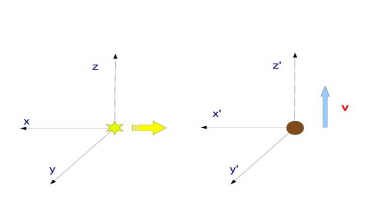
\includegraphics[scale=0.85]{3}
\end{wrapfigure} 

Let's assume that a dust grain is moving respect to the star on a circular orbit (no radial velocity component) with velocity v. The configuration is illustrated in the where the velocity of the grain v is directed along the z'-axis which is parallel to the z-axis of the reference frame centered on the star. A flux of photons leaves the star radially and part of the flux will meet the particle after traveling in the antisolar direction -x. At any instant of time we can assume that the reference frames are inertial with the frame attached to the grain moving with constant velocity along $z\|z'$. This is a good assumption since the absorption and re-emission of energy occurs on a short timescale compared to the circular motion frequency and we do not have to worry about the accelerated circular motion of the grain. We also neglect the fact that both the reference frame are not inertial because that centered on the star is moving under the effect of the dust gravitational attraction. However, the acceleration is so small that can be safely neglected. 

The radiation flux of photons can be described by the momentum 4-vector:
\begin{align}
\label{52}
    p=
    \begin{pmatrix}
    E/c \\
    -E/c \\
    0 \\
    0
    \end{pmatrix}
\end{align}
where we take into account the relation between energy and momentum of a photon $p_x=−E/c$. The minus sign is due to the anti-solar direction of the photon flux. In the reference frame centered on the particle, where absorption and reflection occurs, \textit{p'} is computed by using a Lorentz transformation:
\begin{align}
p'=
    \begin{pmatrix}
    \gamma & 0 & 0 & -\beta\gamma \\
    0 & 1 & 0 & 0 \\
    0 & 0 & 1 & 0 \\
    -\beta\gamma & 0 & 0 & \gamma
    \end{pmatrix}\cdot
    \begin{pmatrix}
    E/c \\
    -E/c \\
    0 \\
    0
    \end{pmatrix}=
    \begin{pmatrix}
    \gamma E/c \\
    -E/c \\
    0 \\
    -\beta\gamma E/c
    \end{pmatrix}
\end{align}
where $\beta=v/c$ and $\gamma=\sqrt{1-v^2/c^2}$.  Now that we have the photon flux in the moving reference frame of the dust grain, we can compute the interaction with the dust particle and, in particular, the momentum absorbed and reflected by the particle:
\begin{align}
    p'_R=
    \begin{pmatrix}
    g\gamma E/c \\
    gE/c \\
    0 \\
    g\beta\gamma E/c
    \end{pmatrix} \quad\quad\quad\quad
    p'_{RE}=
    \begin{pmatrix}
    f\gamma E/c \\
    0 \\
    0 \\
    0
    \end{pmatrix}
\end{align} 
where $p'_r$ is the reflected momentum and $p'_{RE}$ is the re-emitted one, which, since the rays are emitted radially, the radiation momentum going out in a direction is cancelled out by another one leaving in the opposite way. The total radiation leaving from the particle is the sum of both (remember that $f+g=1$ and $Q_{PR}=1+g$):
\begin{align}
    p'_L=
        \begin{pmatrix}
    \gamma E/c \\
    gE/c \\
    0 \\
    g\beta\gamma E/c
    \end{pmatrix}=
        \begin{pmatrix}
    \gamma E/c \\
    -(1-Q_{PR})E/c \\
    0 \\
    -(1-Q_{PR})\beta\gamma E/c
    \end{pmatrix}
\end{align}
changing back to the Sun's reference frame:
\begin{align}
\label{56}
p'=
    \begin{pmatrix}
    \gamma^2(E/c)-\beta^2\gamma^2(E/c)(1-Q_{PR}) \\
    -(1-Q_{PR})E/c \\
    0 \\
    \beta\gamma^2(E/c)-(1-Q_{PR})\beta\gamma^2 E/c
    \end{pmatrix}
\end{align}
with equations \eqref{52} and \eqref{56} we can calculate the variation of 4-momentum of the dust particle, which is the opposite sign from the radiation's. This time we ignore the 0-index because we are only interested in the momentum:
\begin{align}
\begin{split}
    \Delta p=-(p'-p)&=
    \begin{pmatrix}
    (1-Q_{PR})E/c-E/c \\
    0 \\
    -\beta\gamma^2(E/c)+(1-Q_{PR})\beta\gamma^2 E/c
    \end{pmatrix} \\
    &=\begin{pmatrix}
    -(E/c)Q_{PR} \\
    0 \\
    -\beta\gamma^2(E/c)Q_{PR}
    \end{pmatrix}
\end{split}
\end{align}
considering only the z-direction factor on the last index, $v<<c$ ($\gamma^2=1$) and substituting the value of $\beta$, Poynting-Roberson drag is finally:
\begin{align}
    F_{PRD}=-\frac{\textbf{v}}{c^2}EQ_{PR}
\end{align}
which is oriented towards the negative direction of the particle's velocity. The radiation pressure is given by the x-axis in the index 1 of (57):
\begin{align}
    F_{SR}=-(E/c)Q_{PR}
\end{align}
which is oriented outwards of the radial direction. 

Note that, in the past calculations of the drag, we consider energy \textit{E} as a potency, hence it is already divided by time, since \textit{S}'s unit is $W/m^2$ and the product of \textit{S} and \textit{A} is given by Watt (equation 43).

The P-R drag contributes to the decrease of semi-major axis and eccentricity. Solar winds contribute to P-R drag but it is negligibly. 

Radiation pressure force has a $1/r^2$ dependence hidden in the radiation flux S and, as a consequence, its effect is that of weakening the gravitational attraction of the star. Dividing the modulus of equation (59) (with $E=S_0A/r^2$) by the modulus of the Sun's gravitational pull, we obtain the parameter $\beta$:
\begin{align}
    \beta=\frac{F_R}{F_G}=\frac{S_0Q_{PR}Ar^2}{cGMmr^2}=\frac{S_0Q_{PR}(\pi s^2)}{cGM(4\pi s^2\rho/3)}=\frac{3S_0Q_{PR}}{4cGM\rho}
\end{align}
if the dust particle is on a given orbit, its orbital elements will be constants but the orbital period will be longer and the orbital velocity slower. If instead the dust particle is emitted from a body on a given orbit (like a comet because of outgassing) then the orbital elements of the grain can be significantly different from those of the parent body and the grain can also be ejected on a hyperbolic orbit. Let's assume that the dust grain is ejected when the comet is at perihelion by a comet with semi-major axis a and eccentricity e. When the grain is part of the parent body, its orbital energy (which must be negative to be tied to the star) is given by the kinetic minus the gravitational energies:
\begin{align}
\begin{split}
    E&=\frac{1}{2}v^2-\frac{\mu}{r} \\
    v^2\,(\textrm{at pericenter})=\frac{\mu}{a}(\frac{1+e}{1-e})\implies E&=\frac{\mu}{2a}(\frac{1+e}{1-e})-\frac{\mu}{r} \\
    r\,(\textrm{at pericenter})=a(1-e)\implies E&=\frac{\mu}{2a}(\frac{1+e}{1-e})-\frac{\mu}{a(1-e)}
    \end{split}
\end{align}
with $m=1$ because the dust mass is very small, and $\mu=GM$. During the ejection, the kinetic term does not change much, but we have a impact on gravitational one thanks to the solar pressure, so we subtract $\mu$ by the reduced fraction $-\mu\beta$:
\begin{align}
\begin{split}
    E&=\frac{\mu}{2a}(\frac{1+e}{1-e})-\frac{\mu(1-\beta)}{a(1-e)} \\
    E&=\frac{\mu}{2a(1-e)}(1+e-2+2\beta) \\
    E&=\frac{\mu}{2a(1-e)}(e-1+2\beta)
\end{split}
\end{align}
if the term $(e-1+2\beta)$ becomes larger than 0 because of the presence of $\beta$ then the particle escapes the gravitational attraction of the star.

\begin{wrapfigure}{l}{0.5\textwidth}
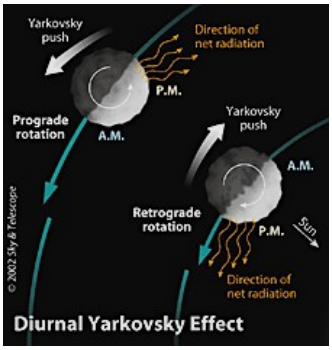
\includegraphics[scale=0.85]{4}
\end{wrapfigure}

For bodies much bigger than dust particles, the non-homogeneous heating of the body can provoke a new drag force. When the body carries on its own rotation, the half that faces the Sun, which re-emits much more than the obscured half, moves sideways, and its produced recoil pushes the body inwards or outwards, where push orientation depends on the rotation direction. This is called as the Yarkovsky effect. The diurnal effect happens when rotation axis is perpendicular to orbital plane, and seasonal effect when the axis is inside the plane.

To obtain the force per mass unit of the body, we relate in a formula the momentum from $E/c=\sigma T^4/c$, the emissivity $\epsilon$, which tells how much the body emits in the infrared, the factor 2/3, which refers to how much radiation is re-emitted perpendicularly to the body's surface, and finally the mass \textit{m}, and we integrate everything by \textit{ds}:
\begin{align}
    \textbf{f}=-\frac{2}{3}\frac{\epsilon\sigma}{mc}\int_sdsT^4\hat{n}
\end{align}
Considering that we do not know about the structure of the body, we will not be able to discover the temperature through the Fourier equation ($F=k\Delta T$, where k is a constant that depends on the body's composition). We can adopt a simplified equation that relates the effect to the variation of semi-major axis:
\begin{align}
    \frac{da}{dt}_{diurnal}&=\frac{8\alpha\pi R^2\epsilon_0}{9nmc}F_\omega(R,\theta)cos\gamma \\
    \frac{da}{dt}_{seasonal}&=\frac{4\alpha\pi R^2\epsilon_0}{9nmc}F_n(R,\theta)sin^2\gamma
\end{align}
where $\alpha$ is the albedo and $\gamma$ is the obliquity. The functions F describe the heating propagating in the body.

The near-Earth asteroids are those that populate the region inside the asteroid belt. The primordial ones are speculated to be extinct by colliding with the Sun in 20 Myrs time spam. They usually have a very elliptical and chaotic orbit which cannot be described like a keplerian orbit, thanks to the disruptive gravitational fields of the solar system. Asteroids can be injected inside the near-Earth region from the asteroid belt when affected by inward drifts or collisions.
\vspace{10mm}

\section{Non-gravitational Forces (March 31st)}
    
Circunstellar and debris disk are different. While the first is composed by gas (H and He) and dust on accretion process of planetesimals and quicker dissipation, the second is made by dust produced in collisions of a planetesimals.

Circunstellar disks have a lifetime of 5 to 10 Myr, which was discovered by observing how the disks in a population of stars evolve with time. Mass of the star is also another important factor of disk evolution, where the more massive ones tend to dissipate faster at the beginning and slower at older ages.

The powerlaw density, temperature and superficial distributions are give by:
\begin{align}
    \begin{split}
        \rho(r)=\rho_0r^{-\alpha} \\
        T(r)=T_0r^{-\beta} \\
        \sigma_d(r)=\sigma_{d0}r^{-\gamma}
    \end{split}
\end{align}
where $\rho_0$, $T_0$ and $\sigma_{d0}$ are the initial values from the first age of the disk. The gas drag, where the disk causes friction on the planetesimals, happens when the angular velocities from both bodies are different. Writing the centripetal acceleration as keplerian motion minus force due to pressure:
\begin{align}
\begin{split}
    a_g=\frac{v^2}{r}=\frac{\omega^2_gr^2}{r}=r\omega_g^2 \\
    r\omega^2_g=\frac{GM}{r^2}-F(P)
\end{split}    
\end{align}
substituting the keplerian angular velocity:
\begin{align}
    \begin{split}
        \omega_k=(\frac{GM}{r^3})^{1/2} \\
        r\omega^2_g=r\omega^2_k-F(P)
    \end{split}
\end{align}
now we consider that pressure is applied on both sides of a slab of dimensions dx, dy and dz, where on one side it is given as P(x) and on the other as P(x+$\delta$x). Starting from the difference of pressure, we multiply it by area to obtain the net force and finally divide by volume to find the force density:
\begin{align}
    \begin{split}
        \Delta P&=-P(x+\delta x) +P(x) \\
        F&=[-P(x+\delta x)+P(x)]\,dydz \\
        F/V&=[-P(x+\delta x)+P(x)]\,\frac{dydz}{dxdydz} \\
        F/V&=-\frac{\partial P}{\partial x}
    \end{split}
\end{align}
substituting Newton's law on the left-hand side and exposing acceleration:
\begin{align}
\begin{split}
    F/V&=\frac{ma}{V}=\rho a \\
    a&=-\frac{1}{\rho}\frac{\partial P}{\partial x}
\end{split}
\end{align}
finally substituting it in (68):
\begin{align}
    r\omega^2_g=r\omega^2_k+\frac{1}{\rho}\frac{\partial P}{\partial r}
\end{align}
to obtain an expression for $\omega_k$ we start from the ideal gas equation and substitute density and temperature from (66):
\begin{align}
\begin{split}
    PV=nRT \implies P&=\frac{nN_AmRT}{VN_Am}=\frac{\rho KT}{m} \\
    &=\frac{K}{m}\rho_0T_0r^{-\alpha}r^{-\beta}
    \end{split}
\end{align}
deriving by \textit{r}:
\begin{align}
    \frac{dP}{dr}=-\frac{K}{m}\rho_0T_0r^{-\alpha-\beta-1}(\alpha+\beta)=-(\alpha+\beta)\frac{K}{m}\frac{\rho T}{r}
\end{align}
substitute back into (71) and exposing $\omega_g$:
\begin{align}
\begin{split}
r\omega^2_g&=r\omega^2_k-(\alpha+\beta)\frac{K}{m}\frac{T}{r} \\
\omega^2_g&=\omega^2_k-(\alpha+\beta)\frac{K}{m}\frac{T}{r^2}
\end{split}
\end{align}
substituting $\omega_k$ from (68) and factoring both right-hand terms in relation to it:
\begin{align}
    \begin{split}
        \omega^2_g&=\frac{GM}{r^3}(1-(\alpha+\beta)\frac{K}{m}\frac{T}{r^2}\frac{r^3}{GM}) \\
        &=\frac{GM}{r^3}(1-(\alpha+\beta)\frac{KT}{m}\frac{r}{GM}) \\
        &=\frac{GM}{r^3}(1-2\eta(r))
    \end{split}
\end{align}
where $\eta (r)$ is equal to the negative term inside the parenthesis. This allows us to conclude that the gas is orbiting slower than the keplerian orbit. We can derive the value of $\eta$ by relating the mean thermal speed $C_m$ with keplerian velocity (68):
\begin{align}
\begin{split}
    C_m&=\sqrt{\frac{8KT}{\pi \mu M_H}} \\
    \eta&=\frac{\pi}{16}(\alpha+\beta)\frac{C_m^2}{\omega_k^2} \\
    \eta&=\frac{\pi}{16}(\alpha+\beta)\frac{8KT}{\pi\mu m_H}\frac{r^3}{GM} \\
    \eta&=\frac{1}{2}(\alpha+\beta)\frac{KT}{m}\frac{r}{GM}
\end{split}
\end{align}
where $m_H$ is the mass of hydrogen atom and $\mu$ is the dimensionless mean molecular weight. In conclusion, the gas moves according with factor $\eta$, which depends on $C_m$ and $\omega_k$ and constants of radial distribution $\alpha$ and $\beta$.

Epstein drag law is responsible for explaining the pull of dust particles smaller than the gas mean free path, which are locked in higher plane orbits by the gas pressure, that slowly settle into the disk plane where the planetesimal formation occurs. To start, let us calculate the number of gas particles which collide with the dust particle:
\begin{align}
    N=vdt\frac{\pi s^2\rho}{\mu m_H}
\end{align}
where $vdt$ is the length of a cylinder which confines the gas. We multiplied by $\pi/s^2$ to obtain volume, and then by $\rho/\mu m_H$ to obtain the number $N$. The velocity is divided into thermal and drift. For the first velocity, only 1/3 of its magnitude contributes to collisions which represents the modulus in the dust particle's direction, and the second velocity refers to the gas's motion relative to the dust. We then insert these velocities and calculate the frequency of collision:
\begin{align}
    f=(\frac{1}{3}v_{th}+v)\frac{\pi s^2\rho}{\mu m_H}\frac{dt}{dt}=(\frac{1}{3}v_{th}+v)\frac{\pi s^2\rho}{\mu m_H}
\end{align}
now we write the same, but for the particles hitting from the opposite direction, hence $v$ is negative:
\begin{align}
    b=(\frac{1}{3}v_{th}-v)\frac{\pi s^2\rho}{\mu m_H}
\end{align}
the tranfer of momentum to the dust is:
\begin{align}
    \Delta p=-\frac{2}{3}v_{th}\mu m_H
\end{align}
where we ignore drift velocity because its modulus is negligible if compared the thermal one. Now, considering the momentum transfer from gas on the other side, we calculate the the total transfer:
\begin{align}
\begin{split}
    \Delta p_T&=(f-b)\Delta p \\
    &=[(\frac{1}{3}v_{th}+v)-(\frac{1}{3}v_{th}-v)]\frac{\pi s^2\rho}{\mu m_H}\cdot(-\frac{2}{3}v_{th}\mu m_H) \\
    F_D&=-\frac{4}{3}v_{th}v\pi s^2\rho
\end{split}
\end{align}
which is the \textbf{Epstein drag force}, and we can consider it as a resistive force $\textbf{F}=f\textbf{v}$. The velocity solution from the equation for free fall in resistive mean is:
\begin{align}
\begin{split}
    ma&=F-fv \\
    v(t)&=\frac{F}{f}(1-e^{-ft/m})
\end{split}
\end{align}
when time scalates, the value of $e$ goes to zero, and our formula becomes $v(t)=F/f$. Substituting \textit{f} from (81), the gravitational force as $F=GMz/r^3$, and then the mass of gas $m$ by $4\pi s^3\rho/3$:
\begin{align}
\begin{split}
    v(t)&=\frac{GMmz/r^3}{\frac{4}{3}\pi s^2v_{th}\rho_g} \\
    &=\frac{\frac{4}{3}GMz\pi s^3\rho_d}{\frac{4}{3}\pi s^2v_{th}\rho_g r^3} \\
    &=\frac{GMz\rho_d s}{v_{th}\rho_g r^3}
\end{split}
\end{align}
if we express the gravity force in function of the keplerian frequency, we get:
\begin{align}
    \Omega_k^2=\frac{GM}{r^3}\implies v(t)=\frac{\Omega_k^2z\rho_d s}{v_{th}\rho_g}
\end{align}
with this, we can calculate the time in which the dust takes to travel from the z height and settle on the middle of the disk plane:
\begin{align}
    t=\frac{z}{v_{set}}=\frac{v_{th}\rho_g}{\Omega_k^2\rho_d s}
\end{align}
this time is expected to be $10^5$ yrs.

After the dust settles and starts to form the planetesimals, its particles become bigger than the gas' free mean path, making the gas pressure lose relevance and giving place to the gravity field. That's where the Stokes drag law comes into place. The gas now is just a fluid that flows through the planetesimal's surface, and its drag is described by:
\begin{align}
    \Vec{F_D}=-\frac{C_D}{2}\pi s^2\rho_gv\Vec{v}
\end{align}
where $C_D$, the drag coefficient, depends on Reynold's number which is:
\begin{align}
    R=\frac{2sv}{\nu_m}
\end{align}
where $\nu_m$ is the viscosity, s is the typical length of motion and v is the relative fluid velocity. By decomposing Stokes drag into radial, tangent and vertical directions, we see that it has a final effect of circularizing orbits, lowering inclination and bringing planetesimals closer to the star, hence making them more stable. It also keeps the relative velocity among planetesimals low, preventing destructive collisions and then speeding up evolution. The gas fluid can also explain the formation of chondrules, which are formed when planetesimals are locked into mean motion resonance and create shock waves that heat up the silicate rocks.

The planetary system of a binary star is divided by S-type and P-type orbits. In the first one, planets orbit an individual planet, and in the second one they orbit the baricenter of the binary system. The perturbation of another star can create high relative velocities, but the gas drag is very important when it comes to stabilize them.

\textbf{Possible exam topics:} proof of the velocity difference between gas and keplerian, and therefore the $\eta$ parameter; proof of Epstein law; proof of dust settling time; effects of the Stokes law in the planetesimal evolution.
\vspace{10mm}

\section{Orbital elements (April 3rd)}

We start by studying the 2-body problem. We have the bigger mass $m_1$ and the smaller one $m_2$. $\Vec{F}_1$ is the gravitational force on $m_1$ and $\Vec{F}_2$ is the opposite, negative force on $m_2$. The distance from reference frame $O$ to $m_1$ is $\Vec{r}_1$ and from $O$ to $m_2$ is $\Vec{r}_2$, while the distance between both masses is $\Vec{r}$, which is equal to $\Vec{r}_2-\Vec{r}_1$. That means that the double derivative, or the acceleration, is given by:
\begin{align}
\begin{split}
    \Ddot{r}&=\Ddot{r_2}-\Ddot{r_1} \\
    &=(-\frac{Gm_1m_2}{r^3m_2}-\frac{Gm_1m_2}{r^3m_1})\Vec{r} \\
    &=-\frac{G(m_1+m_2)}{r^3}\Vec{r} 
\end{split}
\end{align}
\begin{wrapfigure}{l}{0.5\textwidth}
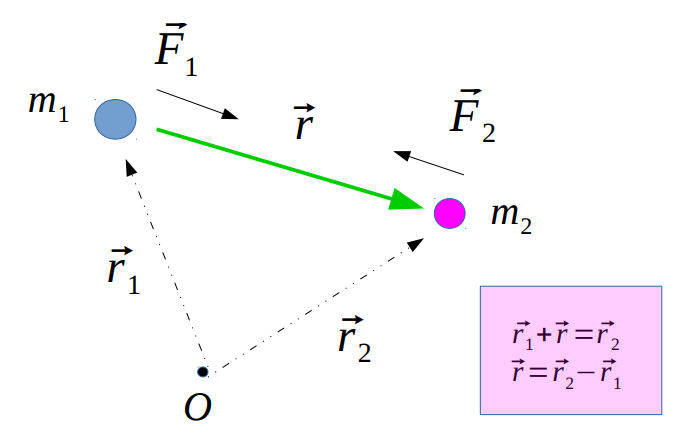
\includegraphics[scale=0.4]{5}
\end{wrapfigure}
then, let us introduce the parameter $\mu$ and include it in equation (88):
\begin{align}
    \mu&=-G(m_1+m_2) \\
    0&=\Ddot{r}+\mu\frac{\Vec{r}}{r^3}
\end{align}
we define the angular momentum as:
\begin{align}
    \Vec{h}=\Vec{r}\times\Vec{\dot{r}}
\end{align}
which does not include mass because it is negligible. In polar coordinates, we have:
\begin{align}
    \Ddot{r}=(\Ddot{r}-r\dot{\theta}^2)\hat{r}+[\frac{1}{r}\frac{d}{dt}(r^2\dot{\theta})]\hat{\theta}
\end{align}
equalizing with (90) into terms related to $\hat{r}$ and $\hat{\theta}$:
\begin{align}
    (\Ddot{r}-r\dot{\theta}^2)+\mu\frac{\Vec{r}}{r^3}&=0 \\
    \frac{1}{r}\frac{d}{dt}(r^2\dot{\theta})&=0
\end{align}
we see that the $\hat{\theta}$ term is equal to zero because equation (90) has no dependence on it, and considering that in the left-hand we have the derivative of $r^2\dot{\theta}$, we assume that $r^2\dot{\theta}$ is a constant, which is equal to the modulus of angular momentum if we transform it into polar coordinates:
\begin{align}
    \Vec{h}=r\hat{r}\times(\dot{r}\hat{r}+r\dot{\theta}\hat{\theta})=r^2\dot{\theta}\hat{z}
\end{align}
solving the equation (93) for $r(\theta)$:
\begin{align}
\begin{split}
    r(\theta)=\frac{p}{1+ecos(\theta-\theta_0)} 
\end{split}
\begin{split}
    \textrm{where:} \;  p=\frac{h^2}{\mu}
\end{split}
\end{align}
which describes, in polar coordinates, the trajectory of a minor body around a massive one. Since we are dealing with a conic equation, which is divided into ellipses, parabolas and hyperbolas, we take our preference for the elliptical conics as it is the one that describes the orbital motion, in which we have:
\begin{align}
\begin{split}
    p&=a(1-e^2)  \\
    h&=\sqrt{\mu a(1-e^2)}
\end{split}
\begin{split}
    \textrm{where:} \;  e<1
\end{split}
\end{align}
where $p$ is the distance between the focus and the orbital position located on the same vertical line, and $a$ is the semi-major axis. $f$ is called as the true anomaly, which is the angle between the pericenter and the current position of the body. The distance between center and focus is $ae$. Apocenter $q$, which is the farthest distance in the orbit, and semi-minor axis $b$ are:

\begin{wrapfigure}[7]{r}{0.45\textwidth}
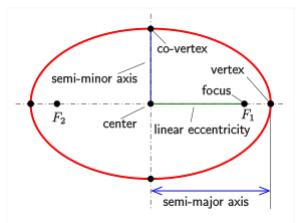
\includegraphics[scale=0.9]{6}
\end{wrapfigure}
\begin{align}
    q=a(1+e) \\
    b=a\sqrt{1-e^2}
\end{align}

Now we must find the trajectory under a time dependence. Let us define the areal velocity, which is the variation of area over time, starting from the area of an angular section $d\theta$:
\begin{align}
\begin{split}
    A=\frac{1}{2}(r\cdot r d\theta) \implies v_r=\frac{1}{2}r^2 \dot{\theta}=\frac{1}{2}h
\end{split}
\end{align}
multiplying $v_r$ by period $T$ we get the area of the ellipse, which is given by $A=\pi ab$. Substituting (99), (100) and then (97) in it:
\begin{align}
\begin{split}
    v_rT&=\pi ab=\pi a^2\sqrt{1-e^2} \\
    T&=\frac{2\pi a^2\sqrt{1-e^2}}{\sqrt{\mu a(1-e^2)}}=2\pi\sqrt{\frac{a^3}{\mu}}=2\pi n
\end{split}
\end{align}
here we also define the mean motion parameter $n$, also known as the frequency of the orbit:
\begin{align}
    n=\sqrt{\frac{a^3}{\mu}}
\end{align}
the mean anomaly $M$ is the fraction of elapsed time during the orbit in relation to total period:
\begin{align}
    M=n(t-t_0)
\end{align}
we can define the system's constant of total energy, including kinetic and potential ones, as:
\begin{align}
    \frac{1}{2}v^2-\frac{\mu}{r}=-\frac{\mu}{2a}
\end{align}

\begin{wrapfigure}[10]{l}{0.35\textwidth}
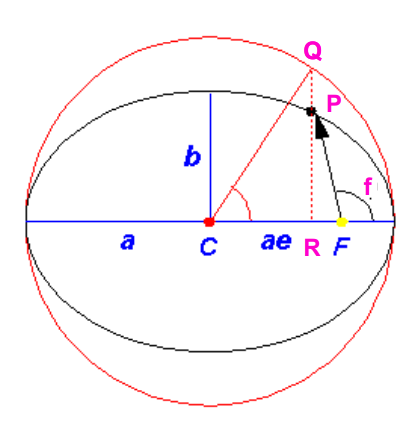
\includegraphics[scale=0.5]{7}
\end{wrapfigure}
where we ignore the mass $m$. Note that the energy is a function of semi-major axis. The eccentric anomaly $U$ is the angle between semi-major axis and the line that goes from the center to the point $Q$ of a fictitious circular orbit, which is centered in the same origin than the ellipse's, located in the same vertical line than the current position $P$ (consult the image below). We can also settle some other distances inside the orbit:
\begin{align}
    FR&=rcosf=acosU-ae \\
    PR&=rsinf =\sqrt{1-e^2}asinU \\
    r&=a(1-ecosU) \\
    tg(\frac{f}{2})&=(\frac{1+e}{1-e})^{1/2}tg(\frac{U}{2})
\end{align}
where now we have $r$ and $f$ as a function of $U$. Deriving U over time and solving its time dependence:
\begin{align}
    \frac{dU}{dt}=\frac{n}{(1-ecosU)} \\
    U-esinU=nt=M
\end{align}
where (110) is the Kepler equation. If we solve it for $U$, then substitute it in (108) and solve for true anomaly ($f=\theta-\theta_0$), and finally substitute it in (97) we can solve $r(t)$ with:
\begin{align}
    r(t)=\frac{a(1-e^2)}{1+cosf}
\end{align}
we can solve Kepler equation using the iterative method, which is good in solving low eccentricity orbits. We start with an initial value $U_0$ and calculate its value after every time step $t-t_0$:
\begin{align}
\begin{split}
    U_0&= M \\
U_1&=U_0+e sin U_0 \\
U_2&=U_0+e sin U_1 \\
\dots\\
U_{i+ 1}&=U_0+e sinU_i
\end{split}
\end{align}
or else we use Newton-Raphson method, which has a faster convergence than the iterative one. We start with a guess for $U_0$ and calculate a corrected value $U_1$ closer to the real one, then we keep iterating until we get to the lowest acceptable $\delta$. Delta is obtained from the Taylor expansion until the second term of the function $f(U_0+\delta)$:
\begin{align}
\begin{split}
    f(U_0+\delta)&=f(U_0)+f'(U_0)\cdot\delta+\dots=0 \\
    \delta&=-\frac{f(U_0)}{f'(U_0)} \\
    U_1&=U_0+\delta
\end{split}
\end{align}

\begin{wrapfigure}[10]{l}{0.4\textwidth}
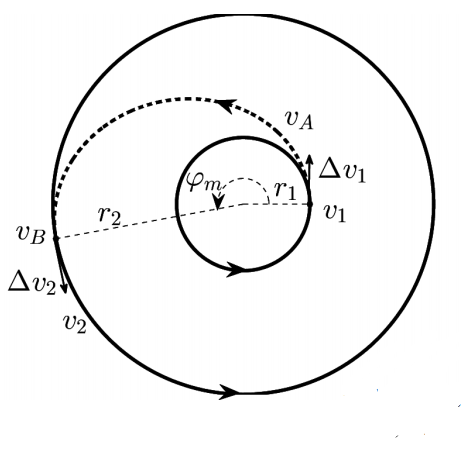
\includegraphics[scale=0.5]{8}
\end{wrapfigure}
Let us now calculate the Hohmann transfer, in which we transfer a satellite from a shorter orbit with radius $r_1$ to a larger $r_2$. These radius are equivalent to parameters of pericenter distance (distance between focus and perihelium) and $q$ (98), respectively. Then, if we sum them together and divide both by 2 we obtain the semi-major axis $a$. We also obtain eccentricity from eq. (97):
\begin{align}
    r_1&=a(1-e) \\
    r_2&=a(1+e ) \\
    a&=\frac{r_1+r_2}{2} \\
    e&=1-\frac{r_1}{a}
\end{align}
now we calculate the velocity difference $\Delta v$ which launches the satellite from small orbit to the elliptical, temporary one. For that, we go back to equation of total energy (104), and expose $v$:
\begin{align}
    v^2=2(\frac{\mu}{r}-\frac{\mu}{2a})=\mu(\frac{2}{r}-\frac{1}{a}) \implies v=\sqrt{\mu(\frac{2}{r}-\frac{1}{a})}
\end{align}
in the small orbit $r=a$, and in the elliptical one the pericenter is $r_1=a(1-e)$, so that means that $\Delta v_1$ is:
\begin{align}
\begin{split}
    v_{1}&=\sqrt{\frac{\mu}{r_1}} \\
    v_{e1}&=\sqrt{\mu(\frac{2}{a(1-e)}-\frac{1}{a})}=\sqrt{\frac{\mu}{a}(\frac{1+e}{1-e})} \\
    \Delta v_1&=v_{e1}-v_1
\end{split}
\end{align}
after the satellite reaches the aphelion there is another change of velocity. The speeds in the aphelium for the elliptical and $r2$ circular orbits, and their $\Delta v_2$ are:
\begin{align}
\begin{split}
    v_e&=\sqrt{\frac{\mu}{a}(\frac{1-e}{1+e})} \\
    v_{2}&=\sqrt{\frac{\mu}{r_2}} \\
    \Delta v_2&=v_2-v_{e2}
\end{split}
\end{align}

We can transform the orbital elements into cartesian vectors and vice-versa:
\[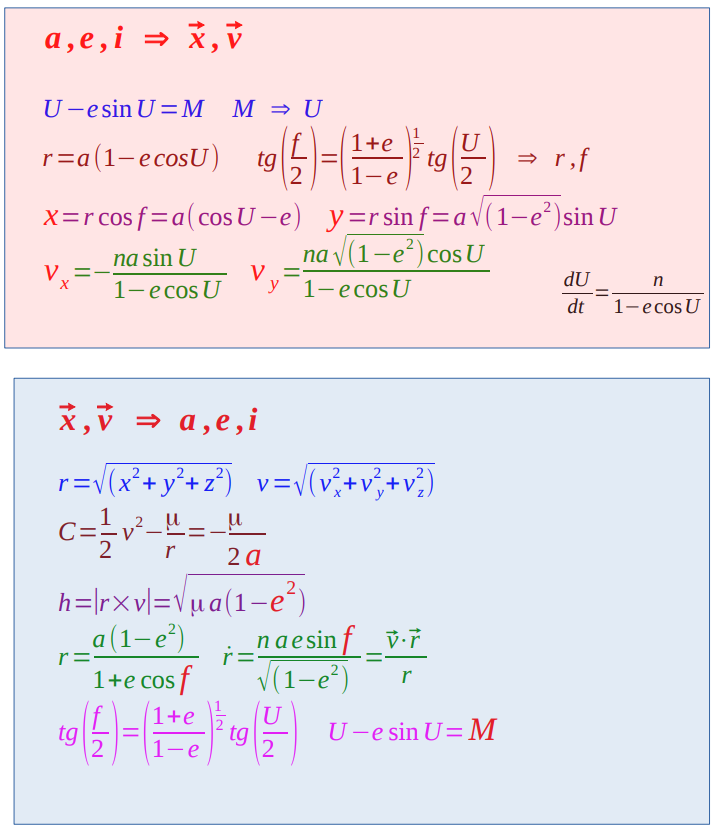
\includegraphics[scale=0.56]{9}\]
in the first scheme we start from $M$ to obtain $U$ (110), with which we find $r$ (107) and $f$ (108), and then $\Vec{r}$ (105) (106) and $\Vec{v}$. Second scheme shows us how we can calculate vectors $\Vec{r}$ and $\Vec{v}$ to achive the values of $a$ (104), $e$ (97), $r$ (111) and $M$ (110).

Let us introduce 3 new parameters which refer to rotation: pericenter argument $\omega$, inclination $i$ and node longitude $\Omega$, represented by the transformation matrix $M_1$, $M_2$ and $M_3$, respectively. We calculate rotations of 2D position matrix in the following way:
\[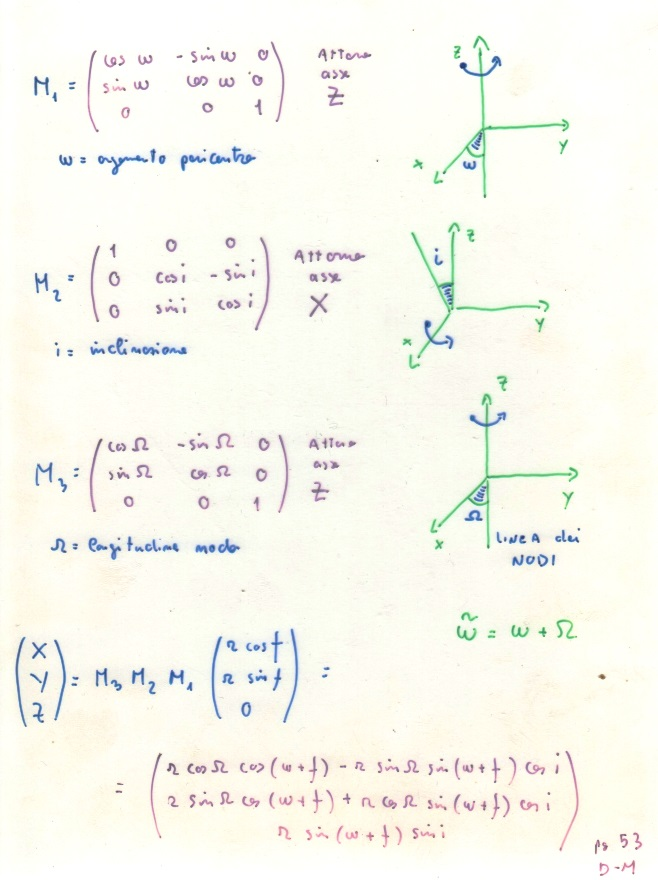
\includegraphics[scale=0.75]{10}\]
remembering that $M_1$, $M_2$ and $M_3$ are not interchangeable and must be computed in the exact same order. With these orbital parameters we can finally obtain a proper result for the actual position and velocity vectors, along $a$, $e$ and $i$ parameters. Having parameters to describe orbits is much more practical than vectors because, except for $M$ which is time dependent, all of them are constants. So all we have to do is calculate the time evolution $M=n(t-t_0)$ to obtain $\Vec{x}$ and $\Vec{v}$.

Knowing the position and velocity vectors, we can find the rotation parameters:
\[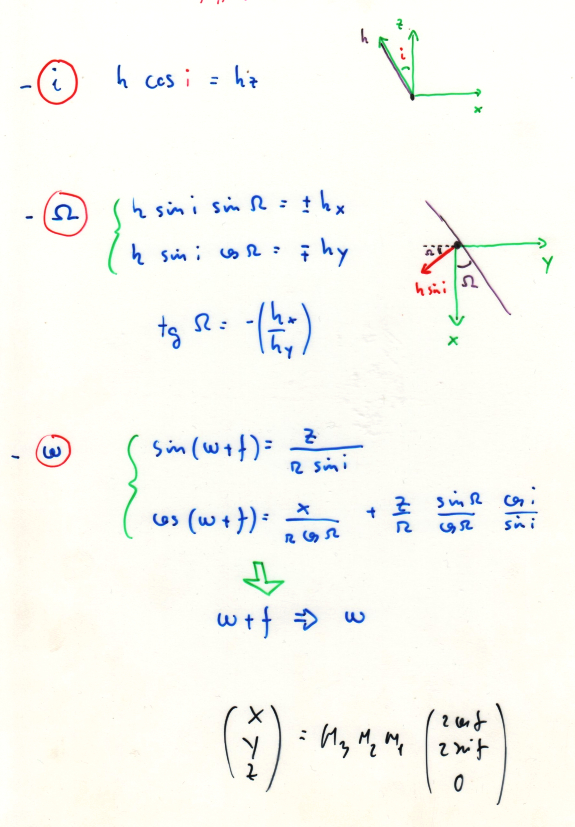
\includegraphics[scale=0.55]{11}\]
first we find $i$ from $h$ and $h_z$ trigonometric relation given by the cosine of $i$. For $\Omega$, we calculate it from the projections of $h$ on the $x$ and $y$ axis. $\omega$ we obtain from the rotation transform matrix.

For last, we compute the baricenter position in the baricenter reference frame.
\[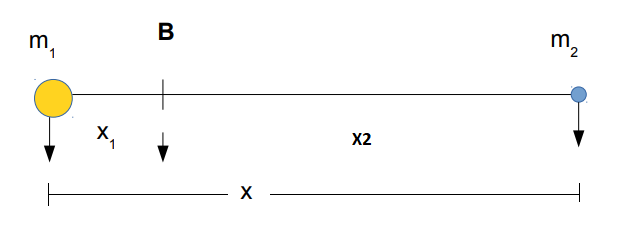
\includegraphics[scale=0.7]{12}\]

Consider $x$ as total distance between bodies, $x_1$ as the distance between larger body $m_1$ and baricenter and $x_2$ as distance between minor body $m_2$ and baricenter, which implies that $x_2=x-x_1$ and $x_1=x-x_2$. We can write the center of mass as:
\begin{align}
\begin{split}
    -m_1x_1+m_2(x-x_1)=0 \\
    x_1=\frac{m_2}{m_1+m_2}x
\end{split}
\begin{split}
    -m_1(x-x_2)+m_2x_2=0 \\
    x_2=\frac{m_1}{m_1+m_2}x
    \end{split}
\end{align}
interpreting $x_1$ and $x_2$ as radial distances from the baricenter, we can relate it to angular momentum (95):
\begin{align}
\begin{split}
    R_1^2\dot{\theta}=(\frac{m_2}{m_1+m_2})^2R^2\dot{\theta}=(\frac{m_2}{m_1+m_2})^2h=h_1 \\
    R_2^2\dot{\theta}=(\frac{m_1}{m_2+m_1})^2R^2\dot{\theta}=(\frac{m_1}{m_2+m_1})^2h=h_2
\end{split}    
\end{align}
where $R^2\dot{\theta}$ is the value of $h$ for the old reference frame of $m_2$ in relation to $m_1$, while $R_1^2\dot{\theta}$ and $R_2^2\dot{\theta}$ refers to the value of $h$ for $m_1$ and $m_2$ in relation to baricenter. The total angular momentum $L$ is given by the sum of $h_1$ multiplied by $m_1$ with $h_2$ multiplied by $m_2$ (we now include the masses, since $h$ is independent of them), from which we also obtain the system's energy:
\begin{align}
    L&=m_1h_1+m_2h_2=\frac{m_1m_2}{m_1+m_2}h \\
    E&=-\frac{Gm_1m_2}{2a}
\end{align}
with this we make a comparison between reference frames through equations (89), in which we have a summation instead of product of masses, and (97), where we have a different value of $h$.
\vspace{10mm}

\section{Non-gravitational Forces (April 7th)}





\end{document}